% !TeX program = xelatex
\documentclass[UTF8,a4paper,11pt,fontset=fandol]{ctexart}
\usepackage[margin=18mm]{geometry}
\usepackage{graphicx,booktabs,tabularx,array,xcolor}
\usepackage[colorlinks=true,urlcolor=blue]{hyperref}
\setlength{\parindent}{0pt}
\setlength{\parskip}{3pt}
\renewcommand{\arraystretch}{1.08}
\pagestyle{plain}
\newcommand{\code}[1]{\texttt{\detokenize{#1}}}
\begin{document}
{\Large\bfseries Ada 渐进量化：曲线与中间结果}\hfill{\small 2026-10-13}

{\small
版本：piR2 \code{11d9ddb + progressive patch}；RTX 6000 Ada，Spatial checkpoint-500。\\
范围：VLM 所选 Linear 固定 W8A8；DiT 192 个候选位置分 11 档转为 W4A4；仅固定重放，未验证闭环质量。\\
计时：每配置 90 次完整本地 plan 调用；GPU sum 为另行 profile 的 6 次 plan 均值，两者不可相减求 CPU 耗时。
}

\begin{center}
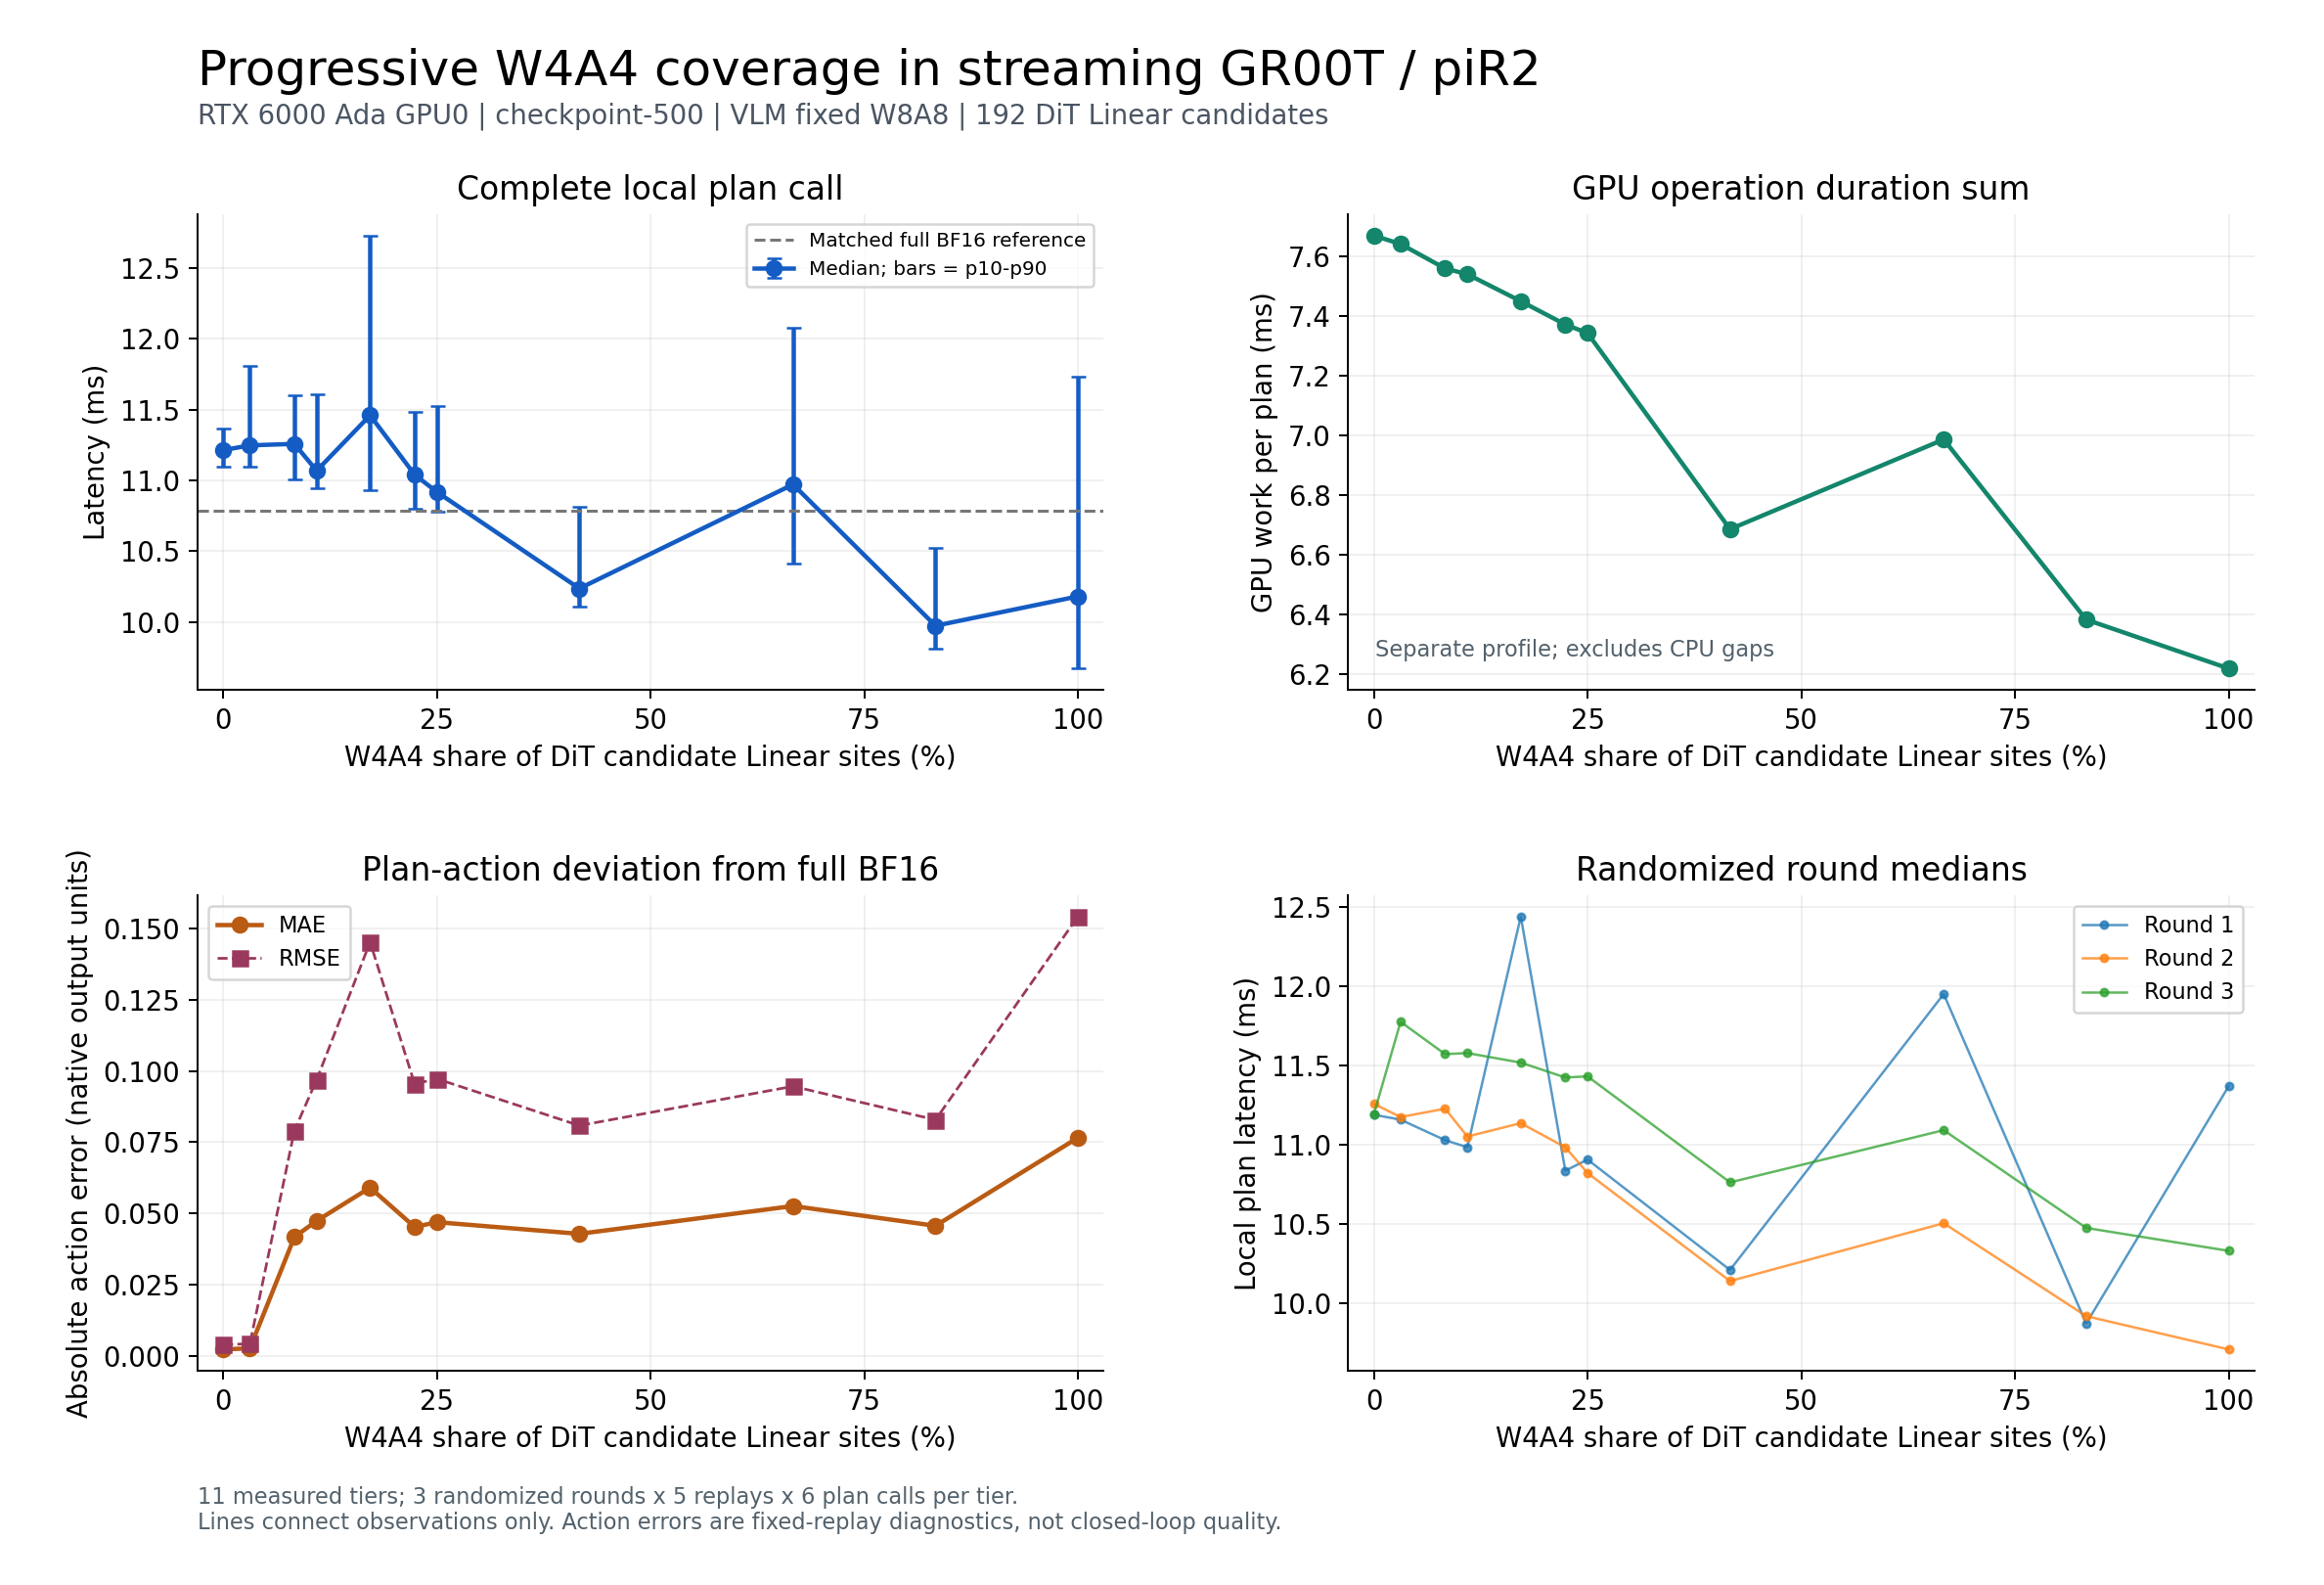
\includegraphics[width=\linewidth,height=0.62\textheight,keepaspectratio]{ada_progressive_curve.png}
\end{center}
\vspace{-3mm}
{\small 连线只连接观测点；误差棒为样本 p10--p90，并非置信区间。三轮重复同一序列，不是独立任务样本。}

\begin{center}\small
\begin{tabular}{lrrr}\toprule
配置 & DiT W4 覆盖率 & plan 中位数（ms） & GPU sum 均值（ms）\\\midrule
BF16 参考 & --- & 10.789 & 8.205\\
T0 & 0\% & 11.213 & 7.671\\
T7 & 41.7\% & 10.237 & 6.685\\
T8 & 66.7\% & 10.971 & 6.987\\
T9 & 83.3\% & 9.974 & 6.382\\
T10 & 100\% & 10.181 & 6.218\\\bottomrule
\end{tabular}
\end{center}
{\small 全 11 档及动作误差见 \code{ada_tiers.csv}；调用级样本见 \code{ada_latency_samples.csv}（共 1080 条）。T9 仅为合并样本中位数最低，不能认定稳定最优。}

\clearpage
{\Large\bfseries DiT 算子拆分与可复用附件}

\begin{center}
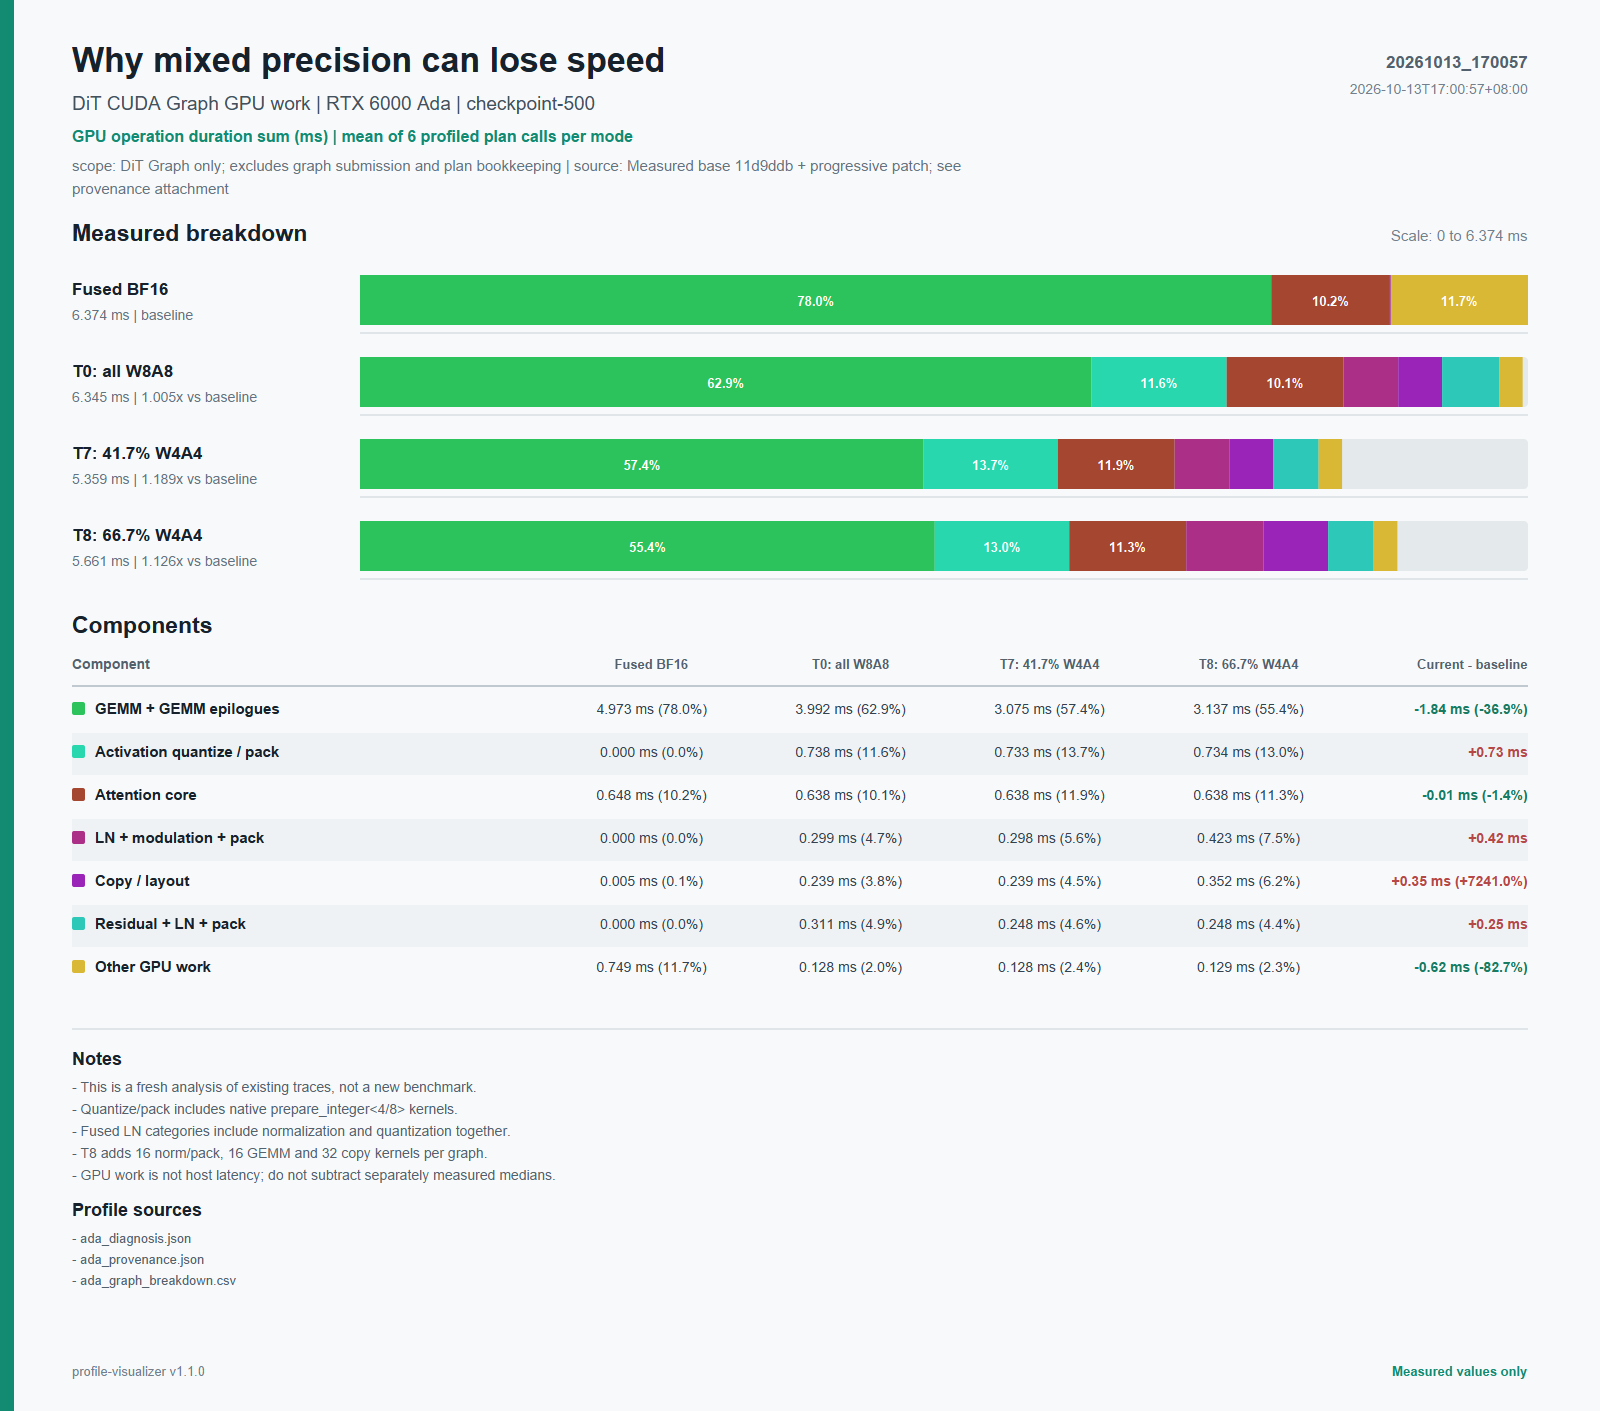
\includegraphics[width=\linewidth,height=0.52\textheight,keepaspectratio]{ada_operator_breakdown.png}
\end{center}
\vspace{-3mm}
{\small 图中数值为 DiT Graph 内 GPU 操作累计，来自每配置 6 次单独 profile 的均值。}

\begin{center}\small
\begin{tabularx}{\linewidth}{Xr}\toprule
实测变化 & 差额（ms）\\\midrule
BF16 $\rightarrow$ W8A8：DiT GEMM 及收尾 & $-0.981161$\\
BF16 $\rightarrow$ W8A8：其余 DiT GPU 操作 & $+0.952067$\\
BF16 $\rightarrow$ W8A8：DiT GPU 合计 & $-0.029094$\\
T7 $\rightarrow$ T8：整个 plan GPU 操作合计 & $+0.301307$\\
T7 $\rightarrow$ T8：完整 plan 墙钟中位数 & $+0.734693$\\\bottomrule
\end{tabularx}
\end{center}
{\small
T8 的 Q/K/V 位宽为 4/4/8；每 Graph 比 T7 多 16 个归一化/打包、16 个 GEMM、32 个复制 kernel。代码与 trace 支持分组拆分和重复准备输入的机制；未做独立消融，不能把墙钟增量全部归于 GPU sum 增量。\\
动作偏差包含 VLM 量化影响；不是纯 DiT 误差，也不是闭环成功率。
}

\vspace{2mm}
{\bfseries 附件索引}\par
{\footnotesize
\code{ada_tiers.csv}、\code{ada_rounds.csv}、\code{ada_latency_samples.csv}：逐档、逐轮和调用级数据。\\
\code{ada_graph_breakdown.csv}、\code{ada_graph_counts.csv}、\code{ada_t7_t8_delta.csv}：算子累计、计数与 T7/T8 增量。\\
\code{ada_selected_sites.json}、\code{ada_diagnosis.json}：实际位宽映射、投影组和 trace 归集。\\
\code{ada_provenance.json}、\code{ada_validation_summary.json}：版本与哈希、测量范围及测试边界。\\
\code{ada_reproducibility.zip}：源码补丁、重放入口、说明及去私有路径的测试日志。
}
\end{document}
